\chapter{Background}\label{chap:background}
\section{JavaScript} \label{sec:background-javascript}
JavaScript is the standard programming language for developing client-side web applications. Together with HTML and CSS, they conform the key technology stack of the Web.

JavaScript is compliant with the ECMAScript Language Specification \citep{ecma-script}. It is an interpreted, dynamically typed language that allows to program small scripts very fast.  Its low learning curve, the possibility of fast prototyping and its easy interaction with the browser's DOM made it the ideal programming languages for introducing dynamic behavior to web applications.

Numerous JavaScript frameworks that aid the development of web applications have been created over the years. \mintinline{text}{jQuery} is used by 74.2\% of the 10 million most popular websites, making it the most popular JavaScript framework in the market \citep{jquery}\citep{w3techs-javascript-libraries-statistics}. Other frameworks like \mintinline{text}{AngularJS}, \mintinline{text}{React} and \mintinline{text}{Vue.js} appeared as an elegant alternative for building complex and scalable web applications \citep{angularjs}\citep{react}\citep{vuejs}. A very simple example of how to use \mintinline{text}{jQuery} for adding dynamic behavior to a web page is shown in \coderef{code:background-jquery-example}.

\begin{code}
	\htmlcode{code/background/javascript/jquery-example.html}
	\captionsetup{aboveskip=0pt, belowskip=10pt}
	\caption[Example using JavaScript and HTML]{\textbf{Example using JavaScript and HTML} - Very simple example that uses library jQuery to hide an element from the DOM when it gets clicked. The example was extracted from W3Schools website.}
	\label{code:background-jquery-example}
\end{code}

All browsers have built-in interpreters that support running JavaScript code. The language is also used to develop backend applications that run in server side runtime environments like NodeJS \citep{nodejs}.

\figref{fig:background-survey-programming-languages} shows that it is the most popular programming languages among professional developers. Additionally, 5 of the 12 most popular frameworks used for web developing are JavaScript frameworks. Similarly, it can be seen in \figref{fig:background-programming-languages-evolution} that JavaScript's popularity remained constant in the last 3 years while being the most popular programming language for seven consecutive years.


\begin{figure}[tp]
	\centering
	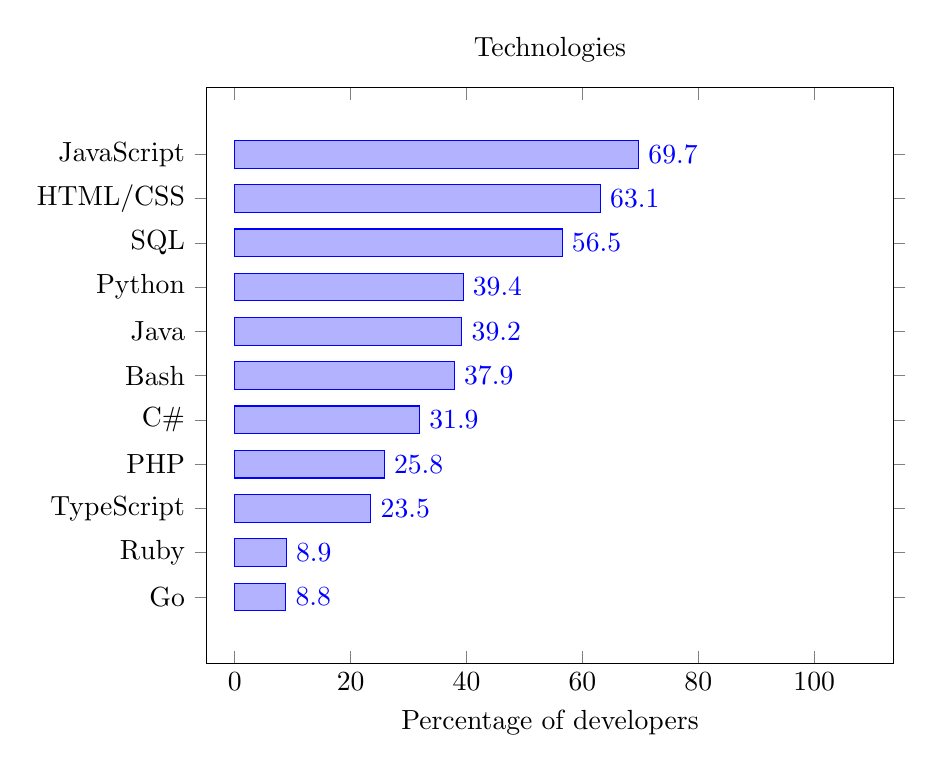
\begin{tikzpicture}
		\begin{axis}[
			xbar,
			title=Technologies,
			width=0.85\textwidth,
			xbar=0pt,
			xmax=100,
			enlargelimits=0.15,
			legend style={at={(0.5,-0.2)}, anchor=south,legend columns=-1},
			xlabel=Percentage of developers,
			symbolic y coords={
				Go,
				Ruby,
				TypeScript,
				PHP,
				C\#,
				Bash,
				Java,
				Python,
				SQL,
				HTML/CSS,
				JavaScript,
			},
			ytick=data,
			nodes near coords, 
			y tick label style={anchor=east},
			every axis plot/.append style={
				bar shift=0pt,
				fill
			  }
		]
		\addplot coordinates {
			(69.7,JavaScript)
			(63.1,HTML/CSS)
			(56.5,SQL)
			(39.4,Python)
			(39.2,Java)
			(37.9,Bash)
			(31.9,C\#)
			(25.8,PHP)
			(23.5,TypeScript)
			(8.9,Ruby)
			(8.8,Go)
		};
		\end{axis}
	\end{tikzpicture}
	%
	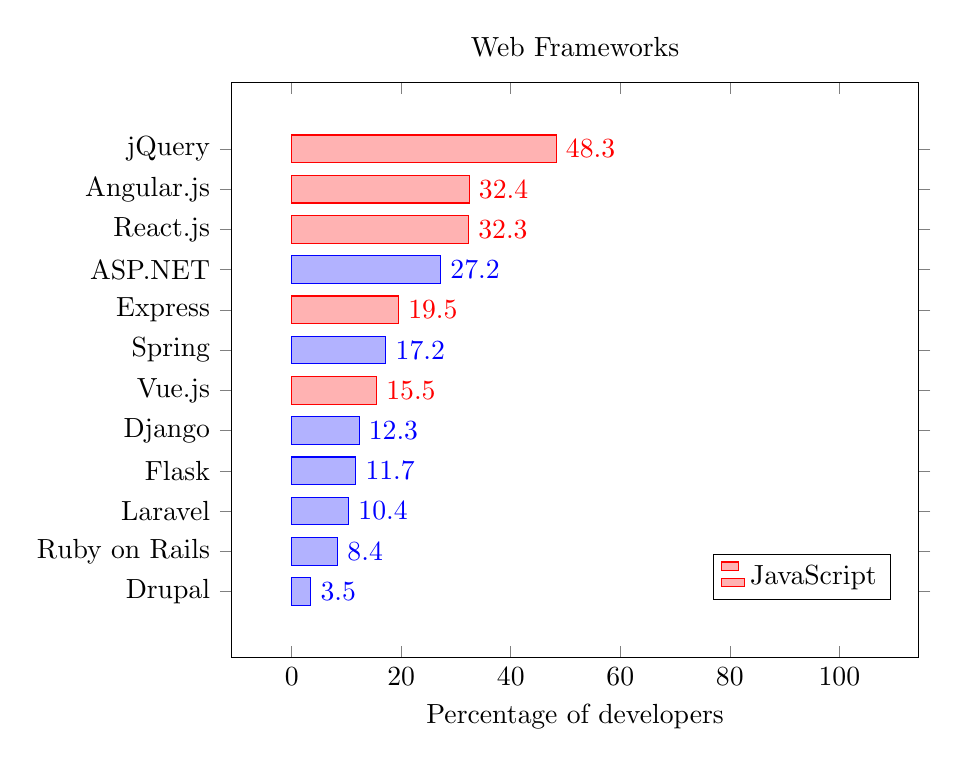
\begin{tikzpicture}
		\begin{axis}[
			xbar,
			title=Web Frameworks,
			width=0.85\textwidth,
			xbar=0pt,
			xmax=100,
			enlargelimits=0.15,
			legend style={at={(0.7,0.1)}, anchor=south west,legend columns=-1},
			xlabel=Percentage of developers,
			yticklabels={
				jQuery,
				Angular.js,
				React.js,
				ASP.NET,
				Express,
				Spring,
				Vue.js,
				Django,
				Flask,
				Laravel,
				Ruby on Rails,
				Drupal,
			},
			ytick={12, 11, ..., 1},
			nodes near coords, 
			y tick label style={anchor=east},
			every axis plot/.append style={
				bar shift=0pt,
				fill
			  }
		]

		\addplot coordinates {
			(27.2,9)
			(17.2,7)
			(12.3,5)
			(11.7,4)
			(10.4,3)
			(8.4,2)
			(3.5,1)
		};

		\addplot coordinates {
			(48.3,12)
			(32.4,11)
			(32.3,10)
			(19.5,8)
			(15.5,6)
		};

		\legend{,JavaScript}
		\end{axis}
	\end{tikzpicture}
	\caption[Conditional operators]{\textbf{Most Popular Technologies \& Frameworks 2019} - According to Stackoverflow's Developer Survey, JavaScript is the most commonly used programming language for 2019. 5 out of 12 of the most popular Web Frameworks are written in JavaScript.
	}
\end{figure}

\begin{figure}[tp]
	\centering
	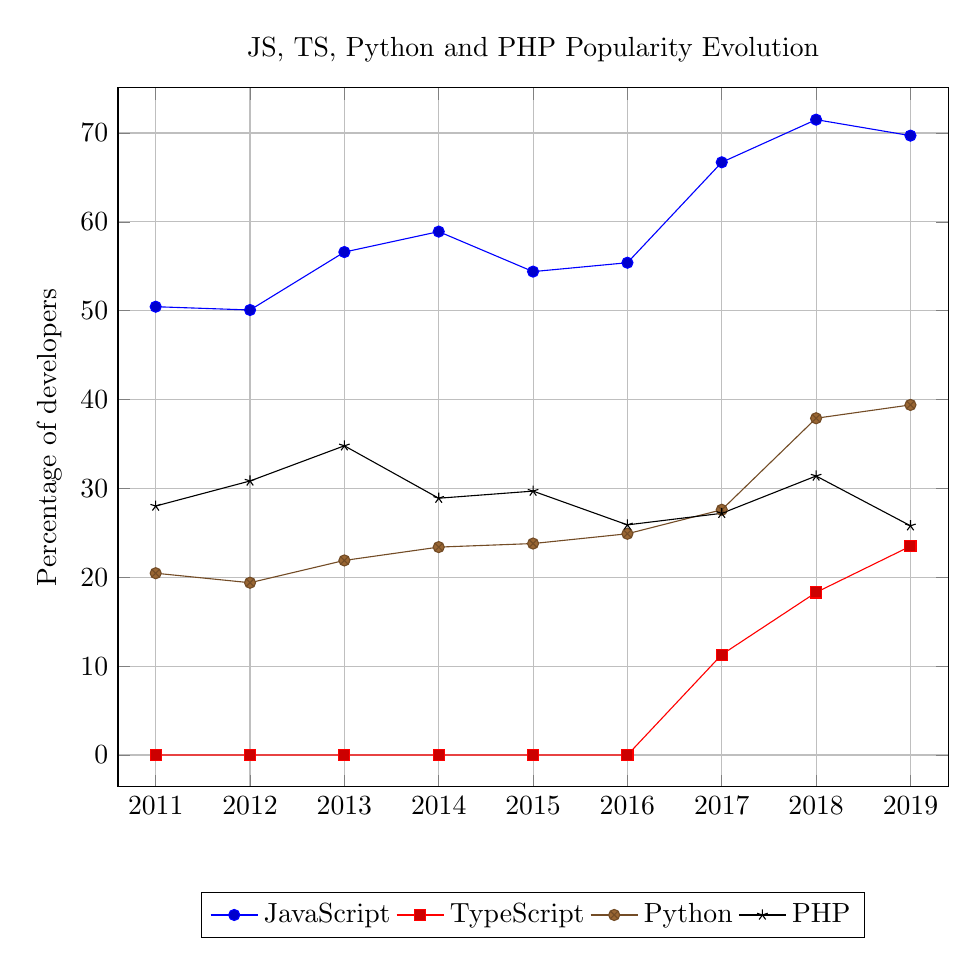
\begin{tikzpicture}
		\begin{axis}[
			width=1\textwidth,
			ylabel=Percentage of developers,
			title={JS, TS, Python and PHP Popularity Evolution},
			enlargelimits=0.05,
			legend style={at={(0.5,-0.15)},
				anchor=north,legend columns=-1},
			xticklabels={
				2011,
				2012,
				2013,
				2014,
				2015,
				2016,
				2017,
				2018,
				2019
			},
			xtick={0,...,8},
			grid=major,
		]

		% JavaScript
		\addplot coordinates {
			(0,50.45)
			(1,50.08)
			(2,56.60)
			(3,58.90)
			(4,54.40)
			(5,55.4)
			(6,66.7)
			(7,71.5)
			(8,69.7)
		};
		
		% TypeScript
		\addplot coordinates {
			(0,0)
			(1,0)
			(2,0)
			(3,0)
			(4,0)
			(5,0)
			(6,11.3)
			(7,18.3)
			(8,23.5)
		};
		
		% Python
		\addplot coordinates {
			(0,20.46)
			(1,19.39)
			(2,21.9)
			(3,23.4)
			(4,23.8)
			(5,24.9)
			(6,27.6)
			(7,37.9)
			(8,39.4)
		};

		% PHP
		\addplot coordinates {
			(0,28.02)
			(1,30.84)
			(2,34.8)
			(3,28.9)
			(4,29.7)
			(5,25.9)
			(6,27.2)
			(7,31.4)
			(8,25.8)
		};
		\legend{JavaScript,TypeScript,Python,PHP}
		\end{axis}
	\end{tikzpicture}
	\caption[Conditional operators]{\textbf{JS, TS, Python and PHP Popularity Evolution 2011 - 2019} - According to Stackoverflow's Developer Survey, for the seventh year in a row, JavaScript is the most commonly used programming language. While JavaScript's popularity remained constant for the last 3 years, TypeScript's popularity is increasing every year. There is no data for TypeScript before 2017.}
\end{figure}

\subsection{Types}
Section 8 of the ECMAScript Language Specification presents the allowed types for a variable \citep{ecma-script}. These are: \mintinline{text}{undefined}, \mintinline{text}{null}, \mintinline{text}{boolean}, \mintinline{text}{string}, \mintinline{text}{number}, \mintinline{text}{object} and \mintinline{text}{symbol} for ES6/ECMAScript 2015. All of them except for \mintinline{text}{object} are called primitives.

It must be noted that functions and arrays are not built-in types. Functions are considered to be `member of the Object type that is an instance of the standard built-in Function constructor and that may be invoked as a subroutine' \citep{ecma-script}. The \mintinline{text}{Function} object is a built-in object with a \mintinline{text}{[[Call]]} internal property, which means that it can be invoked. Similarly, arrays are instances of the built-in \mintinline{text}{Array} object. Both concepts are shown in \coderef{code:background-functions-and-arrays}.

\begin{code}
	\jscode{code/background/javascript/functions-and-arrays.js}
	\captionsetup{aboveskip=0pt, belowskip=10pt}
	\caption[Functions and arrays are built-in objects in JS]{\textbf{Functions and arrays are built-in objects in JS} - A function can be created using the \mintinline{text}{function} keyword or using the \mintinline{text}{Function} built-in constructor. Similarly, arrays can be created using brackets or the \mintinline{text}{Array} built-in object.}
	\label{code:background-functions-and-arrays}
\end{code}

Finally, the \mintinline{text}{typeof} operator is not an exact match with the built-in types. It surprisingly returns \mintinline{text}{'object'} for \mintinline{text}{null}, \mintinline{text}{'function'} for a \mintinline{text}{function} and \mintinline{text}{'object'} for an \mintinline{text}{array}. \coderef{code:background-javascript-typeof} gives some examples about this operator.

\begin{code}
	\jscode{code/background/javascript/javascript-typeof.js}
	\captionsetup{aboveskip=0pt, belowskip=10pt}
	\caption[typeof JavaScript operator]{\textbf{\mintinline{text}{typeof} JavaScript operator} - Examples of the \mintinline{text}{typeof} operator for \mintinline{text}{null}, \mintinline{text}{function} and \mintinline{text}{array}.}
	\label{code:background-javascript-typeof}
\end{code}

\subsection{TypeCoercion} \label{sec:background-js-type-coercion}
Type coercion is the process of converting one type into another one. In JavaScript, a variable can be converted into different types depending on the operator and the value of the other operands. The specific definition can be found in the ECMAScript Language Specification \citep{ecma-script}. The following section will cover the basic forms of type coercion but providing a detailed explanation of how JavaScript converts a variable type into another one for each operator is beyond the scope of this section. It is however intended to give insight about this kind of behavior to show its importance while performing type inference in JavaScript. As a result, specific operator related type coercion is explained only for operator \mintinline{text}{+}.

Finally, there are excellent references regarding JavaScript's Type Coercion, like Kyle Simpson's book `You Don't Know JS: Types \& Grammar' \citep{you-dont-know-js}.

\subsubsection{Types of conversion}
\label{types_of_conversion}
There are two types of type coercion: explicit and implicit \citep{you-dont-know-js}. Explicit type coercion is simply when the developer chooses to convert one type into another one. The developer achieves this by writing a piece of code that shows her intention, as shown in \coderef{code:background-explicit-type-coercion}. This type of coercion is also called type casting \citep{you-dont-know-js}.

\begin{code}
	\jscode{code/background/javascript/type-coercion/explicit-type-coercion.js}
	\captionsetup{aboveskip=0pt, belowskip=10pt}
	\caption[Explicit JavaScript Type Coercion]{\textbf{Explicit JavaScript Type Coercion} - The developer explicitly transforms a type into another one. The return values of \mintinline{text}{String()}, \mintinline{text}{Number()} and \mintinline{text}{Boolean()} are always of type \mintinline{text}{string}, \mintinline{text}{number} and \mintinline{text}{boolean}, respectively.}
	\label{code:background-explicit-type-coercion}
  \end{code}

On the other hand, depending on the operator and the context, JavaScript will perform implicit type transformations automatically. If the developer is not aware of this, she may face some unexpected behavior, as shown in \coderef{code:background-implicit-type-coercion}.

\begin{code}
	\jscode{code/background/javascript/type-coercion/implicit-type-coercion.js}
	\captionsetup{aboveskip=0pt, belowskip=10pt}
	\caption[Implicit JavaScript Type Coercion]{\textbf{Implicit JavaScript Type Coercion} - Examples given by Douglas Crockford in his talk `JavaScript: The Good Parts' at Google\footnote{https://www.youtube.com/watch?v=hQVTIJBZook}.}
	\label{code:background-implicit-type-coercion}
\end{code}

In any case, JavaScript will always convert any value into a primitive value \citep{ecma-script}, regardless of explicit or implicit type coercion. There is no coercion mechanism that results in an \mintinline{text}{object} or a \mintinline{text}{function}.

It is fundamental to understand how a value gets coerced into one of these types. JavaScript mainly performs this by applying one of three so called \mintinline{text}{Abstract Operations} \citep{ecma-script}: \mintinline{text}{ToString()}, \mintinline{text}{ToNumber()} and \mintinline{text}{ToBoolean()}.

The operation \mintinline{text}{ToPrimitive()} is also called within the operators. However, each operator will call either \mintinline{text}{ToString()}, \mintinline{text}{ToNumber()} or \mintinline{text}{ToBoolean()} after calling \mintinline{text}{ToPrimitive()}. This operator will be explained in an independent section.

\subsubsection{ToString}
JavaScript performs this conversion in a very intuitive way, as explained in \coderef{code:background-to-string-operation}. Every primitive gets converted as expected. Objects are converted into strings by calling \mintinline{text}{ToPrimtive()} with \mintinline{text}{hint = string}, as presented in \coderef{code:background-to-string-implementation}.

\begin{code}
	\jscode{code/background/javascript/type-coercion/to-string.js}
	\captionsetup{aboveskip=0pt, belowskip=10pt}
	\caption[ToString implementation]{\textbf{ToString implementation}}
	\label{code:background-to-string-implementation}
\end{code}

\begin{code}
	\jscode{code/background/javascript/type-coercion/string-conversion.js}
	\captionsetup{aboveskip=0pt, belowskip=10pt}
	\caption[ToString operation]{\textbf{ToString operation}}
	\label{code:background-to-string-operation}
\end{code}

\subsubsection{ToNumber}
\coderef{code:background-to-number-operation} presents this type of conversion. Strings and boolean values get converted in the expected way. Moreover, \mintinline{text}{undefined} will be converted into \mintinline{text}{NaN} and \mintinline{text}{null} into \mintinline{text}{0}. Similarly, objects are converted into numbers by calling \mintinline{text}{ToPrimtive()} with \mintinline{text}{hint = number}, as presented in \coderef{code:background-to-number-implementation}.

\begin{code}
	\jscode{code/background/javascript/type-coercion/to-number.js}
	\captionsetup{aboveskip=0pt, belowskip=10pt}
	\caption[ToNumber implementation]{\textbf{ToNumber implementation}}
	\label{code:background-to-number-implementation}
\end{code}

\begin{code}
	\jscode{code/background/javascript/type-coercion/number-conversion.js}
	\captionsetup{aboveskip=0pt, belowskip=10pt}
	\caption[ToNumber operation]{\textbf{ToNumber operation}}
	\label{code:background-to-number-operation}
\end{code}


\subsubsection{ToBoolean}
Only the values presented in \coderef{code:background-to-boolean-operation} are converted into \mintinline{text}{false}. Everything else is coerced to \mintinline{text}{true}. That means, that every non-empty \mintinline{text}{string}, every non-zero \mintinline{text}{number} and every \mintinline{text}{object} gets coerced to \mintinline{text}{true}.

Values that are converted into \mintinline{text}{false}, like \mintinline{text}{null} or \mintinline{text}{undefined} are called \textit{falsy} values \citep{you-dont-know-js}.

\begin{code}
	\jscode{code/background/javascript/type-coercion/boolean-conversion.js}
	\captionsetup{aboveskip=0pt, belowskip=10pt}
	\caption[ToBoolean operation]{\textbf{ToBoolean operation}}
	\label{code:background-to-boolean-operation}
\end{code}

\subsubsection{ToPrimitive}
The signature of this function is \mintinline{text}{ToPrimitive(value, preferredType)}. The allowed values for \mintinline{text}{preferredType} are \mintinline{text}{string} or \mintinline{text}{number}. Every JavaScript operator will try to convert an object into a primitive by invoking \mintinline{text}{ToPrimitive} with a different value for \mintinline{text}{preferredType}. If no value is passed, \mintinline{text}{number} is considered as the default, except for JavaScript native \mintinline{text}{Date} objects, where \mintinline{text}{string} is used as default.

An implementation of this behavior is shown in \coderef{code:background-to-primitive-operation}.

\begin{code}
	\jscode{code/background/javascript/type-coercion/to-primitive/to-primitive.js}
	\captionsetup{aboveskip=0pt, belowskip=10pt}
	\caption[ToPrimitive operation]{\textbf{ToPrimitive operation}}
	\label{code:background-to-primitive-operation}
\end{code}

An important aspect that should be considered, is that the type of the return value of \mintinline{text}{ToPrimitive()} does not necessarily have to match the chosen \mintinline{text}{preferredType}. This means concretely that, for example, you can call \mintinline{text}{ToPrimitive(a, number)} and get a \mintinline{text}{string} as a result. Of course, when performing an explicit type conversion, JS will eventually convert whatever \mintinline{text}{ToPrimitive} returns into the correct type. But some operators will perform different implicit type conversions \textit{after} calling \mintinline{text}{ToPrimitive()}. The specific type conversion will then be dependent on the type of the return value of \mintinline{text}{ToPrimitive()} and not on the chosen \mintinline{text}{preferredType}.

All objects that are converted to \mintinline{text}{boolean} will be coerced to \mintinline{text}{true}. The following paragraphs explain how objects get converted into strings or numbers.

\subsubsection{Object to String}
The object is first converted into a primitive value calling the \mintinline{text}{ToPrimitive()} method, using \mintinline{text}{string} as \mintinline{text}{preferredType}. The obtained primitive value is then normally converted into a \mintinline{text}{string}, as explained before in \coderef{code:background-to-string-implementation}.

\coderef{code:background-object-into-string} shows a straightforward example. On the other hand, \coderef{code:background-object-into-string-not-string-return-value} provides an example where \mintinline{text}{ToPrimitive(val, String)} does not return a \mintinline{text}{string}, either because simply \mintinline{text}{toString()} does not return a \mintinline{text}{string} or because \mintinline{text}{valueOf()} gets being called instead of \mintinline{text}{toString()}.

\begin{code}
	\jscode{code/background/javascript/type-coercion/to-primitive/normal-object-to-string.js}
	\captionsetup{aboveskip=0pt, belowskip=10pt}
	\caption[Object into string conversion]{\textbf{Object into string conversion} - An object has a \mintinline{text}{toString()} method that returns a string.}
	\label{code:background-object-into-string}
\end{code}

\begin{code}
	\jscode{code/background/javascript/type-coercion/to-primitive/object-to-string-returning-not-a-string.js}
	\captionsetup{aboveskip=0pt, belowskip=10pt}
	\caption[Object into string conversion]{\textbf{Object into string conversion} - An object that does not return a \mintinline{text}{string} even though \mintinline{text}{ToPrimitive()} is called with \mintinline{text}{hint = string}.}
	\label{code:background-object-into-string-not-string-return-value}
\end{code}

\subsubsection{Object to Number}
The object gets converted into a primitive by calling \mintinline{text}{ToPrimitive(val, Number)}. Normal number conversion is then applied to this primitive value. \coderef{code:background-object-into-number} provides a basic example. Similarly, \coderef{code:background-object-into-string-not-number-return-value} shows how \mintinline{text}{ToPrimitive()} might return something that is not a \mintinline{text}{number}.

\begin{code}
	\jscode{code/background/javascript/type-coercion/to-primitive/normal-object-to-number.js}
	\captionsetup{aboveskip=0pt, belowskip=10pt}
	\caption[Object into number conversion]{\textbf{Object into number conversion} - An object has a \mintinline{text}{valueOf()} method that returns a \mintinline{text}{number}.}
	\label{code:background-object-into-number}
\end{code}

\begin{code}
	\jscode{code/background/javascript/type-coercion/to-primitive/object-to-number-returning-not-a-number.js}
	\captionsetup{aboveskip=0pt, belowskip=10pt}
	\caption[Object into number conversion]{\textbf{Object into number conversion} - An object that does not return a \mintinline{text}{number} even though \mintinline{text}{ToPrimitive()} is called with \mintinline{text}{hint = number}.}
	\label{code:background-object-into-string-not-number-return-value}
\end{code}

\subsubsection{The \mintinline{text}{+} operator}
If any of the operands is an object, it will first convert it into a primitive by passing no \mintinline{text}{preferredType} to the \mintinline{text}{ToPrimitive()} method. Afterwards, if any value is a \mintinline{text}{string}, this operator will implicitly convert both values into a \mintinline{text}{string} and perform a normal string concatenation between them. Else, it will implicitly convert each value into a \mintinline{text}{number} and perform a normal arithmetic addition. An implementation is presented in \coderef{code:background-plus-operator-implementation}.

\coderef{code:background-plus-operator-simple-examples} shows some basic examples. As explained before and shown in \coderef{code:background-plus-operator-object-example}, \mintinline{text}{ToPrimitive()} may return a \mintinline{text}{string}, even when it is called with no \mintinline{text}{preferredType}. This can happen because:
\begin{enumerate}
	\item \mintinline{text}{valueOf()} is returning a String.
	\item \mintinline{text}{valueOf()} is not returning a primitive, which would make \mintinline{text}{toString()} being called instead.
	\item One of the operands is the native JavaScript \mintinline{text}{Date} Object.
\end{enumerate}

\begin{code}
	\jscode{code/background/javascript/type-coercion/plus-operator-implementation.js}
	\captionsetup{aboveskip=0pt, belowskip=10pt}
	\caption[JavaScript + operator implementation]{\textbf{JavaScript \mintinline{text}{+} operator implementation}}
	\label{code:background-plus-operator-implementation}
\end{code}

\begin{code}
	\jscode{code/background/javascript/type-coercion/plus-operator-simple-examples.js}
	\captionsetup{aboveskip=0pt, belowskip=10pt}
	\caption[JavaScript + operator examples]{\textbf{JavaScript \mintinline{text}{+} operator examples}}
	\label{code:background-plus-operator-simple-examples}
\end{code}

\begin{code}
	\jscode{code/background/javascript/type-coercion/plus-operator-object.js}
	\captionsetup{aboveskip=0pt, belowskip=10pt}
	\caption[JavaScript + operator with object]{\textbf{JavaScript \mintinline{text}{+} operator with object}}
	\label{code:background-plus-operator-object-example}
\end{code}


\subsection{NPM Packages} \label{sec:background-npm-packages}
The Node Package Manager (NPM) is the default package manager for NodeJS, a JavaScript runtime environment built on Google Chrome's V8 JavaScript engine \citep{nodejs}. It offers a public registry where JavaScript libraries can be uploaded to be used by the developer's community.

Dependencies can be installed either globally or as local dependencies of specific a JavaScript projects. NPM installs the dependencies described in the \mintinline{text}{package.json} file and local dependencies are saved in the \mintinline{text}{node_modules} directory in the project's root directory. An example of NPM's usage is shown in \coderef{code:background-npm-usage-example}. The registry contains currently more than 1 million modules and it has 11000 million downloads per week.

\begin{code}
	\begin{bashinline}
$ cat index.js 
const abs = require('abs');
console.log(abs('/foo'));

$ node index.js
Error: Cannot find module 'abs'

$ npm i abs
$ node index.js
/foo
	  \end{bashinline}
	\caption[NPM usage example]{\textbf{NPM usage example} - Requiring the module before installing the dependencies will fail since the library is not available. After installing the dependencies locally under the \mintinline{text}{node_modules} directory, the \mintinline{text}{abs} module can be imported using the \mintinline{text}{require} function.}
	\label{code:background-npm-usage-example}
  \end{code}

\section{TypeScript} \label{sec:background-typescript}
\subsection{Declaration Files} \label{sec:declaration-files-background}
% \todo{Hablar de los tipos de declaration files que hay}
\subsection{Definitely Typed}

\section{Jalangi} \label{sec:jalangi}